\documentclass[a4paper]{article}
\newcommand{\sepspace}{\vspace*{1em}}	
%% Language and font encodings
\usepackage[english]{babel}
\usepackage[utf8x]{inputenc}
\usepackage[T1]{fontenc}

%% Sets page size and margins
\usepackage[a4paper,top=3cm,bottom=2cm,left=3cm,right=3cm,marginparwidth=1.75cm]{geometry}

%% Useful packages
\usepackage{amsmath}
\usepackage{graphicx}
\usepackage[colorinlistoftodos]{todonotes}
\usepackage[colorlinks=true, allcolors=blue]{hyperref}

\title{An opposed-flow methane/air diffusion flame}
\author{Piotr Kieliszek}

\begin{document}
\maketitle



\section{Introduction}

This section will be dedicated to the simulation of a counterflow diffusion flame. Using Cantera program to analize temperature of an opposed-flow methane/air diffusion flame in function of distance from burner with changing temperature, pressure and equivalence ratio.


\section{Mathematic model}

The mixture of methane and air is delivered into burning aerial with total inlet of $0,87kg/m^2/s$ and three parts of experiance are made. In first part the oxidizer temperature is changed from 300K to 400K and finaly 500K and the changes of temperature in function of distance where mesured. In secend part the equivalence ratio is changed from 0,5 to 1,62 and the changes of temperature in function of distance where mesured. In third part the pressure is changed from 100000Pa to 300000Pa and finaly 500000Pa and the changes of temperature in function of distance where mesured.

\section{Backup mathemathic calculations}
\textbf{Calkulations nesesery to find equivalence ratio:}
\[{CH_4 +2(O_2+3,76N_2) }
      = {CO_2+2H_2 O}\] 

274,56g of oxidizer for 16g of fuel in stechiometric condicion so stechiometric FAR(Fuel–air ratio) is $16/274,56=0,058275$. Concentration limits of ignition for methan are 5-15. So limits are 0,05mol(0,8g)of fuel for 0,95mol(27,5215g) of oxidizer and 0,15mol(2,4g)of fuel for 0,85mol(24,6245g) of oxidizer. Finaly limits of equivalence ratio are $0,8/(27,5215*0,058275)=0,49881$ and $2,4/(24,6245*0,058275)=1,67248$

\section{Program description}
\subsection{Basic part of program}

\textbf{Importing libraries}

import cantera as ct

import matplotlib.pyplot as plt

\textbf{Inputing parameters of methane and air}

p = 1e5   \textbf{pressure}

$tin_f = 300.0$   \textbf{fuel inlet temperature}

$tin_o = 300.0$   \textbf{oxidizer inlet temperature}

$mdot_o = 0.82$   \textbf{stechiometric oxidizer inlet $kg/m^2/s$}

$mdot_f = 0.05$   \textbf{stechiometric fuel inlet $kg/m^2/s$}

$comp_o = 'O2:0.21, N2:0.78, AR:0.01'$   \textbf{air composition}

$comp_f = 'CH4:1'$   \textbf{fuel composition}

\textbf{Seting distance between inlets to 2 cm}

$width = 0.02$

\textbf{Seting amount of diagnostic output (0 to 5)}

$loglevel = 1$

\textbf{Createing the gas object used to evaluate all thermodynamic, kinetic, and transport properties.}

$gas = ct.Solution('gri30.xml', 'gri30_mix')$

$gas.TP = gas.T, p$

\subsection{Temperature of flame in function of oxidizer temperature}

\textbf{Createing an object representing the counterflow flame configuration, which consists of a fuel inlet on the left, the flow in the middle, and the oxidizer inlet on the right.}
\hspace{5,35mm}$f = ct.CounterflowDiffusionFlame(gas, width=width)$

\textbf{Seting the state of the two inlets}

$f.fuel_inlet.mdot = mdot_f$

$f.fuel_inlet.X = comp_f$

$f.fuel_inlet.T = tin_f$

$f.oxidizer_inlet.mdot = mdot_o$

$f.oxidizer_inlet.X = comp_o$

$f.oxidizer_inlet.T = tin_o$

\textbf{Seting the boundary emissivities}

$f.set_boundary_emissivities(0.0, 0.0)$

$f.set_refine_criteria(ratio=4, slope=0.2, curve=0.3, prune=0.04)$

\textbf{Solveing the problem}

$f.solve(loglevel, auto=True)$

$f.show_solution()$

$f.save('ch4_diffusion_temp.xml')$

\textbf{writing the velocity, temperature, and mole fractions to a CSV file}

$f.write_csv('ch4_diffusion_temp.csv', quiet=False)$

$f.show_stats(0)$

\textbf{Ploting Temperature with besic parameters}

$figTemperatureModifiedFlame = plt.figure()$

$plt.plot(f.flame.grid, f.T, label=tin_o )$

$plt.title('Temperature of the flame with change of oxidizer temperature')$

$plt.ylim(0,3000)$

$plt.xlim(0.000, 0.020)$

\textbf{Looping whih changes of oxidizer temperaturę from 400 to 500K}

$while tin_o <= 400:$

\hspace{5,35mm}$    tin_o=tin_o+100$

\hspace{5,35mm}$    f.fuel_inlet.T = tin_f$

\hspace{5,35mm}$    f.oxidizer_inlet.T = tin_o$

\hspace{5,35mm}$    f.solve(loglevel=1, refine_grid=False)$

\hspace{5,35mm}$    f.show_solution()$

\hspace{5,35mm}$    plt.plot(f.flame.grid, f.T, label=tin_o)$

\hspace{5,35mm}$    plt.legend()$

\hspace{5,35mm}$    plt.legend(loc=1)$

$plt.savefig('./ch4_diffusion_temperature.pdf')$

\subsection{Temperature of flame in function of equivalence ratio}

\textbf{Reseting besic parameters}

$tin_f=300$

$tin_o=300$

\textbf{Starting from lowest equivalence ratio}

$mdot_f = 0.025$

$mdot_o = 0.87-mdot_f$

$f = ct.CounterflowDiffusionFlame(gas, width=width)$

$f.fuel_inlet.mdot = mdot_f$

$f.fuel_inlet.X = comp_f$

$f.fuel_inlet.T = tin_f$

$f.oxidizer_inlet.mdot = mdot_o$

$f.oxidizer_inlet.X = comp_o$

$f.oxidizer_inlet.T = tin_o$

$f.set_boundary_emissivities(0.0, 0.0)$

$f.set_refine_criteria(ratio=4, slope=0.2, curve=0.3, prune=0.04)$

$f.solve(loglevel, auto=True)$

$f.show_solution()$

$f.save('ch4_diffusion_eq.xml')$

$f.write_csv('ch4_diffusion_eq.csv', quiet=False)$

$f.show_stats(0)$

$figTemperatureModifiedFlame = plt.figure()$

\textbf{Equivalence ratio is calculated in laber inside plt.plot}

$plt.plot(f.flame.grid, f.T, label=mdot_f/(mdot_o*0.058275) )$

$plt.title('Temperature of the flame with change of equivalence ratio')$

$plt.ylim(0,3000)$

$plt.xlim(0.000, 0.020)$

\textbf{Looping whih changed equivalence ratio from 0,5 to 1,62}

$while mdot_f <= 0.065:$

\hspace{5,35mm}$    mdot_f=mdot_f+0.01$

\hspace{5,35mm}$    mdot_o = 0.87-mdot_f$

\hspace{5,35mm}$    f.fuel_inlet.mdot = mdot_f$

\hspace{5,35mm}$    f.oxidizer_inlet.mdot = mdot_o$

\hspace{5,35mm}$    f.solve(loglevel=1, refine_grid=False)$

\hspace{5,35mm}$    f.show_solution()$

\hspace{5,35mm}$    plt.plot(f.flame.grid, f.T, label=mdot_f/(mdot_o*0.058275))$

\hspace{5,35mm}$    plt.legend()$

\hspace{5,35mm}$    plt.legend(loc=1)$

$plt.savefig('./ch4_diffusion_eq.pdf')$

\subsection{Temperature of flame in function of pressure}

$mdot_o = 0.82$

$mdot_f = 0.05$

$f = ct.CounterflowDiffusionFlame(gas, width=width)$

$f.fuel_inlet.mdot = mdot_f$

$f.fuel_inlet.X = comp_f$

$f.fuel_inlet.T = tin_f$

$f.oxidizer_inlet.mdot = mdot_o$

$f.oxidizer_inlet.X = comp_o$

$f.oxidizer_inlet.T = tin_o$

$f.set_boundary_emissivities(0.0, 0.0)$

$f.set_refine_criteria(ratio=4, slope=0.2, curve=0.3, prune=0.04)$

$f.solve(loglevel, auto=True)$

$f.show_solution()$

$f.save('ch4_diffusion_press.xml')$

$f.write_csv('ch4_diffusion_press.csv', quiet=False)$

$f.show_stats(0)$

$figTemperatureModifiedFlame = plt.figure()$

$plt.plot(f.flame.grid, f.T, label=p )$

$plt.title('Temperature of the flame with change of pressure')$

$plt.ylim(0,3000)$

$plt.xlim(0.000, 0.020)$

\textbf{Looping whih changed pressure from 1e5 to 5e5}

$while p <= 3e5:$

\hspace{5,35mm}$    p=p+2e5$

\hspace{5,35mm}$    gas.TP = gas.T, p$

\hspace{5,35mm}$    f = ct.CounterflowDiffusionFlame(gas, width=width)$

\hspace{5,35mm}$    f.fuel_inlet.mdot = mdot_f$

\hspace{5,35mm}$    f.fuel_inlet.X = comp_f$

\hspace{5,35mm}$    f.fuel_inlet.T = tin_f$

\hspace{5,35mm}$    f.oxidizer_inlet.mdot = mdot_o$

\hspace{5,35mm}$    f.oxidizer_inlet.X = comp_o$

\hspace{5,35mm}$    f.oxidizer_inlet.T = tin_o$

\hspace{5,35mm}$    f.set_boundary_emissivities(0.0, 0.0)$

\hspace{5,35mm}$    f.set_refine_criteria(ratio=4, slope=0.2, curve=0.3, prune=0.04)$

\hspace{5,35mm}$    f.solve(loglevel, auto=True)$

\hspace{5,35mm}$    f.show_solution()$

\hspace{5,35mm}$    plt.plot(f.flame.grid, f.T, label=p)$

\hspace{5,35mm}$    plt.legend()$

\hspace{5,35mm}$    plt.legend(loc=1)$

$plt.savefig('./ch4_diffusion_pres.pdf')$


\section{Results}
Program returns diagrams of temperature of an opposed-flow methane/air diffusion flame in function of distance from burner with changing temperature, pressure and equivalence ratio and other data like velocity, mole fractions etc. in CSV format.
\begin{figure}[h!]
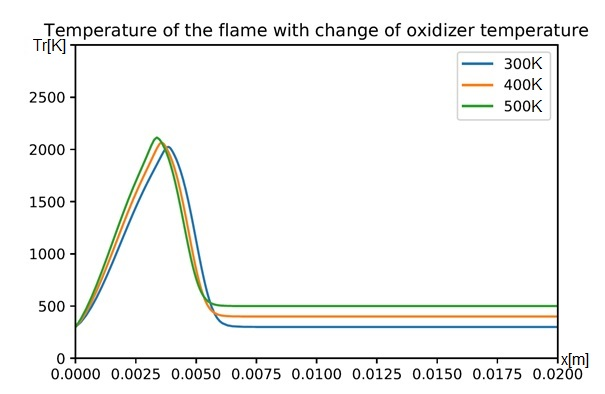
\includegraphics[width=1\textwidth]{1.jpg}
\caption{\label{fig:1}Temperature of an opposed-flow methane/air diffusion flame in function of distance from burner with changing temperature from cantena calculations.}
\end{figure}

\begin{figure}
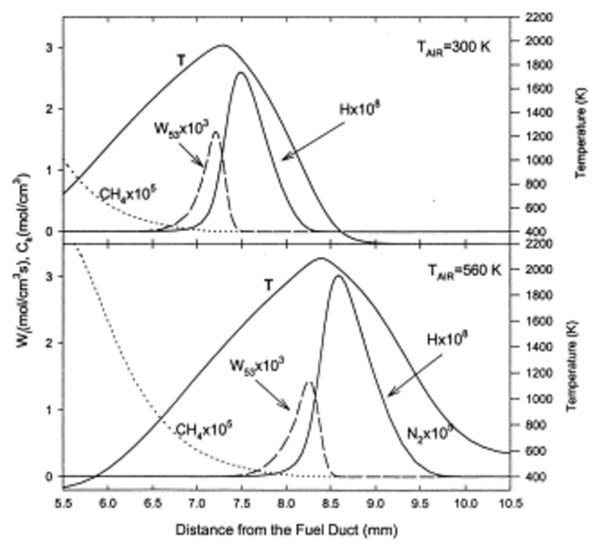
\includegraphics[width=1\textwidth]{2.jpg}
\caption{\label{fig:2}Temperature, $CH_4$, H profiles, and the reaction rate profile for two preheat temperatures.From source [3]}
\end{figure}

\begin{figure}
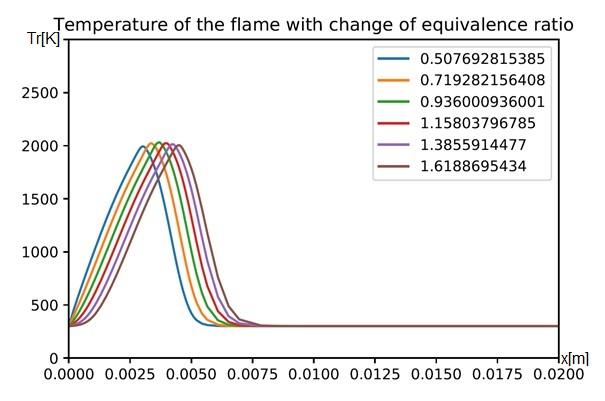
\includegraphics[width=1\textwidth]{3.jpg}
\caption{\label{fig:3}Temperature of an opposed-flow methane/air diffusion flame in function of distance from burner with changing equivalence ratio from cantena calculations.}
\end{figure}

\begin{figure}
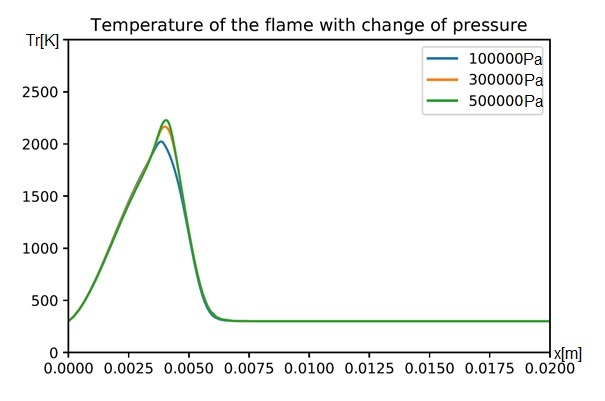
\includegraphics[width=1\textwidth]{4.jpg}
\caption{\label{fig:4}. Temperature of an opposed-flow methane/air diffusion flame in function of distance from burner with changing pressure from cantena calculations .}
\end{figure}

\begin{figure}
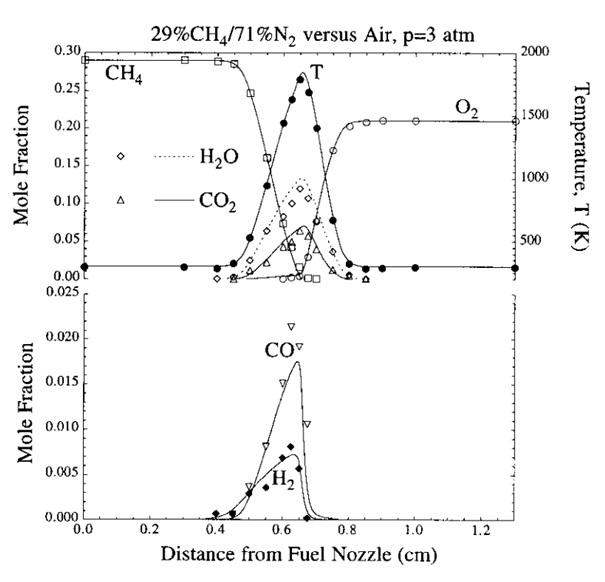
\includegraphics[width=1\textwidth]{5.jpg}
\caption{\label{fig:5}Temperature and mole fraction profiles of the diffusion flames, at 3 atm. From source [4]}
\end{figure}
\section{Conclusions}
Results from calculations for difrent temperatures and pressuresare are close to experimental results for temperature and fractions. Becouse of lack of experimental results for changing equivalence ratio for methane and air mixture it is imposible to comform this calculations but charakter of highest temperaturę points is similar to other gases (highest temperaturę in stehiometry point).
 
\sepspace

\sepspace

\sepspace

\section{References}

$
\hspace{5,35mm}[1] www.cantera.org/docs/sphinx/html/cython/examples/onedim_diffusion_flame.html
$

$
[2] www.sciencedirect.com/science/article/pii/S0082078498805468
$

$
[3] www.sciencedirect.com/science/article/pii/S0010218099001376
$

$
[4] www.sciencedirect.com/science/article/pii/S0082078498805602
$

$
[5] fluid.wme.pwr.wroc.pl/~spalanie/dydaktyka/spalanie_instrukcje/spalanie_labor_instr_stezeniowe
$

\end{document}